%\vspace{1.5pc}
\vspace{1.5pc}
%\section[State of the Art]{State of the Art}
\begin{spacing}{1.5}
	
	Bab ini menjelaskan lebih detail mengenai pustaka relevan dan tinjauan teori dalam penelitian ini. Hal ini bertujuan untuk mereview, mengupdate, mengkritik dan mensintesis literatur, melakukan meta-analisis literatur, melakukan konsepsi ulang dari topik yang direview, dan menjawab pertanyaan spesifik penelitian dari topik yang telah direview dalam literatur \shortcite{Torraco2016}.
	
\end{spacing}
\vspace{-1pc}
\section[Persamaan Primitif]{Persamaan Primitif}
\begin{spacing}{1.5}
	\par Model sirkulasi laut atau \textit{Ocean General Circulation Models} (OGCM) menggunakan persamaan Navier-Stokes untuk memodelkan fenomena fisis yang terjadi di lautan. Lautan adalah fluida yang dapat dijelaskan dengan baik dengan pendekatan persamaan-persamaan primitif, yaitu persamaan Navier-Stokes serta persamaan keadaan nonlinier yang menggabungkan dua variabel (temperatur dan salinitas) dengan kecepatan fluida, dan mempertimbangkan beberapa asumsi dan hipotesis \shortcite{madec_gurvan_2022_6334656}.
	
	Beberapa asumsi yang digunakan dalam persamaan Navier-Stokes diantaranya asumsi Boussinesq, asumsi hidrostatik, dan asumsi tak termampatkan (\textit{incompressibility}). Misalkan $\rho$ sebagai densitas in situ, $T$ sebagai temperatur potensial, $S$ sebagai salinitas, $p$ sebagai tekanan, $z$ sebagai koordinat vertikal, dan $g$ sebagai percepatan gravitasi. Asumsi yang digunakan dalam persamaan Navier-Stokes dapat dituliskan sebagai berikut.\\
	Asumsi Boussinesq
	\begin{equation}\label{eq:P1}
		\rho = \rho(T,S,p).
	\end{equation}
	Berdasarkan asumsi Boussinesq, pengaruh variasi densitas terhadap sistem diabaikan kecuali kontribusinya terhadap gaya apung.\\
	Asumsi hidrostatik
	\begin{equation}
		\frac{\partial p}{\partial z} = -\rho g.
	\end{equation}
	Berdasarkan asumsi hidrostatik, persamaan momentum vertikal direduksi menjadi persamaan kesetimbangan antara variabel gradien tekanan vertikal dan gaya apung.\\
	Asumsi tak termampatkan
	\begin{equation}
		\nabla \;.\; U =\frac{\partial u}{\partial x} + \frac{\partial v}{\partial y} + \frac{\partial w}{\partial z} = 0.
	\end{equation}	
	Berdasarkan asumsi tak termampatkan, persamaan 3-D divergensi untuk vektor kecepatan $U = (u,v,w)$ (dalam koordinat kartesius $(x,y,z)$) dianggap sama dengan 0.
	
	Selanjutnya misalkan $U = U_h + wk$ ($h$ adalah notasi vektor horizontal lokal di atas bidang $(i,j)$). Persamaan vektor invarian (invarian di bawah transformasi koordinat sehingga dapat diterapkan secara seragam dalam sistem koordinat lengkung ortogonal mana pun) dari persamaan primitif dalam sistem vektor $(i, j, k)$ dapat dituliskan dalam persamaan berikut \shortcite{madec_gurvan_2022_6334656}.\\
	Persamaan kesetimbangan momentum
	\begin{equation}\label{eq:P2}
		\begin{aligned}
			\frac{\partial U_h}{\partial t} = - \left[(\nabla \times U) \times U + \frac{1}{2}\nabla (U^2)\right]_h - f \; k \times U_h - \frac{1}{\rho_o}\nabla_h p + D^U + F^U.
		\end{aligned}
	\end{equation}
	Dalam Persamaan (\ref{eq:P2}) di atas, suku $(\nabla \times U) \times U + \frac{1}{2}\nabla (U^2)$ dapat ditulis sebagai $U\cdot \nabla U$ dan merupakan suku percepatan konvektif dari persamaan momentum. Suku $\nabla_h p$ merupakan gradien tekanan, $f = 2\Omega\; \cdot \;k$ merupakan percepatan Coriolis (dengan $\Omega$ adalah vector kecepatan sudut bumi), $D^U$ merupakan parameterisasi dari fisika skala kecil untuk momentum sedangkan $F^U$ merupakan suku gaya permukaan untuk momentum.\\
	Persamaan konservasi panas dan salinitas
	\begin{equation}\label{eq:P3}
		\begin{aligned}
			\frac{\partial T}{\partial t} &= - \nabla \; . \; (T\;U)  + D^T + F^T \\
			\frac{\partial S}{\partial t} &= - \nabla \; . \; (S\;U)  + D^S + F^S,
		\end{aligned}
	\end{equation}
	dengan operator $\nabla$ sebagai vektor turunan yang diperumum dalam arah $(i,j,k)$, variabel $D^T$ dan $D^S$ merupakan parameterisasi dari fisika skala kecil untuk temperatur dan salinitas sedangkan variabel $F^T$ dan $F^S$ merupakan suku gaya permukaan untuk temperatur dan salinitas. 
	 
	Dalam aplikasinya, persamaan Navier-Stokes tidak hanya digunakan untuk memodelkan laut, tapi juga merambah ke bidang pemodelan cuaca \shortcite{Rohli2021}, aliran air dalam pipa \shortcite{Ouchiha2012} dan aliran udara di sekitar sayap pesawat \shortcite{Tulus2019}. Dalam bentuk persamaan lengkap dan simplifikasi, persamaan ini juga dapat digunakan untuk mendesain kereta api \shortcite{Croquer2020}, pesawat terbang \shortcite{Chau2021}, dan mobil \shortcite{Ambarita2018}. Terdapat juga studi tentang aliran darah \shortcite{Gill2021}, desain stasiun pembangkit listrik \shortcite{Yang2019}, dan analisis polusi udara \shortcite{Issakhov2022}. 
	
\end{spacing}
\vspace{-0.1pc}

\section[Model Iklim]{Model Iklim}
\begin{spacing}{1.5}
	Aplikasi deret waktu (\textit{time series}) banyak melibatkan data yang menunjukkan siklus musiman. Contoh yang paling umum digunakan adalah data cuaca. Dalam penelitian \shortciteauthor{Haridhi2016} \citeyear{Haridhi2016}, model nonlinear regresi digunakan untuk mengkarakterisasi hubungan antara SST (\textit{sea surface temperatur}) dan ND (\textit{net deployment}) - penyebaran jaring nelayan pukat cincin tradisional. Untuk menvalidasi temuan ini, mereka menggunakan persamaan siklus musiman \citeA{crawley2012r} dan mencari korelasi antara data SST dan data meteorologi. Dilain hal, \shortciteauthor{Ikhwan2022} \citeyear{Ikhwan2022} dalam penelitiannya mengkaji tentang kedalaman lapisan campuran (MLD) di laut Andaman menggunakan data salinitas (SSS) dari model 3-D CMEMS (\textit{Copernicus Marine Environment Monitoring Service}). Model iklim digunakan untuk mengidentifikasi dan memvalidasi jumlah musim MLD dalam setahun. 
%	Persamaan regresi non-linear \shortcite{Haridhi2016} diformulasikan sebagai
%	\begin{equation}\label{eq:nrl}
%		y = b_1 + b_2(\sin(b_3t+b_4)),
%	\end{equation}
%	dengan $b_1$ adalah konstanta pergeseran vertikal, $b_2$ adalah amplitudo gelombang sinus, $b_3$ adalah frekuensi, $t$ adalah variabel waktu, dan $b_4$ adalah fase.
%	
	Misalkan sebuah titik bergerak dengan kecepatan konstan pada suatu lingkaran dengan jari-jari $\rho$ dan $t$ adalah waktu yang dihitung saat jari-jari terhubung dengan titik pusat pada sudut $\theta$ dibawah sumbu horizontal. Jika titik tersebut diproyeksikan pada sumbu horizontal maka jarak proyeksi dari titik pusat dapat dituliskan sebagai
	\begin{equation}\label{eq:MIK1}
		x = \rho \cos(\omega t-\theta),
	\end{equation}
	dengan $\rho$ adalah amplitudo, $\omega$ adalah kecepatan sudut atau frekuensi, dan $\theta$ adalah perpindahan fase. Gerakan proyeksi bolak-balik sepanjang sumbu horizontal digambarkan sebagai gerak harmonik sederhana.
	
	Kecepatan sudut diukur dalam radian per satuan periode, kuantitas $2\pi / \omega$ adalah periode siklus. Pergerakan fase, juga diukur dalam radian, menunjukkan sejauh mana fungsi kosinus telah berpindah oleh pergeseran sepanjang waktu. Jadi, alih-alih puncak fungsi terjadi pada waktu $t = 0$, seperti yang terjadi pada fungsi kosinus biasa, sekarang terjadi pada
	waktu $t = \theta/\omega$. Selanjutnya perhatikan bahwa $\cos(A-B) = \cos(A)\cos(B)+\sin(A)\sin(B)$, akibatnya persamaan (\ref{eq:MIK1}) dapat ditulis menjadi
	\begin{equation}
		\begin{aligned}
			x &= \rho \cos(\theta)\cos(\omega t) + \rho \sin(\theta)\sin(\omega t) \\
			&= \alpha\cos(\omega t) + \beta\sin(\omega t),
		\end{aligned}
	\end{equation}
	dengan 
	\begin{equation*}
		\alpha = \rho \cos(\theta), \quad 
		\beta = \rho \sin(\theta), \quad \text{dan} \quad
		\alpha^2 + \beta^2 = \rho^2.
	\end{equation*}

	\noindent Persamaan untuk siklus musiman \shortcite{crawley2012r} dapat dituliskan sebagai
	\begin{equation}\label{eq:sm_}
		y = \alpha + \beta \sin(2\pi t)+\gamma \cos(2\pi t) + \epsilon,
	\end{equation}
	dengan $\alpha$ adalah konstanta pergesaran vertikal, $\beta$ adalah amplitudo dari gelombang sinus, $\gamma$ adalah amplitudo dari gelombang kosinus, $t$ adalah waktu, dan $\epsilon$ adalah elemen residual yang mewakili komponen \textit{white-noise} tidak beraturan dalam proses pengambilan data. 
	
	\begin{figure}[H]
		\centering
		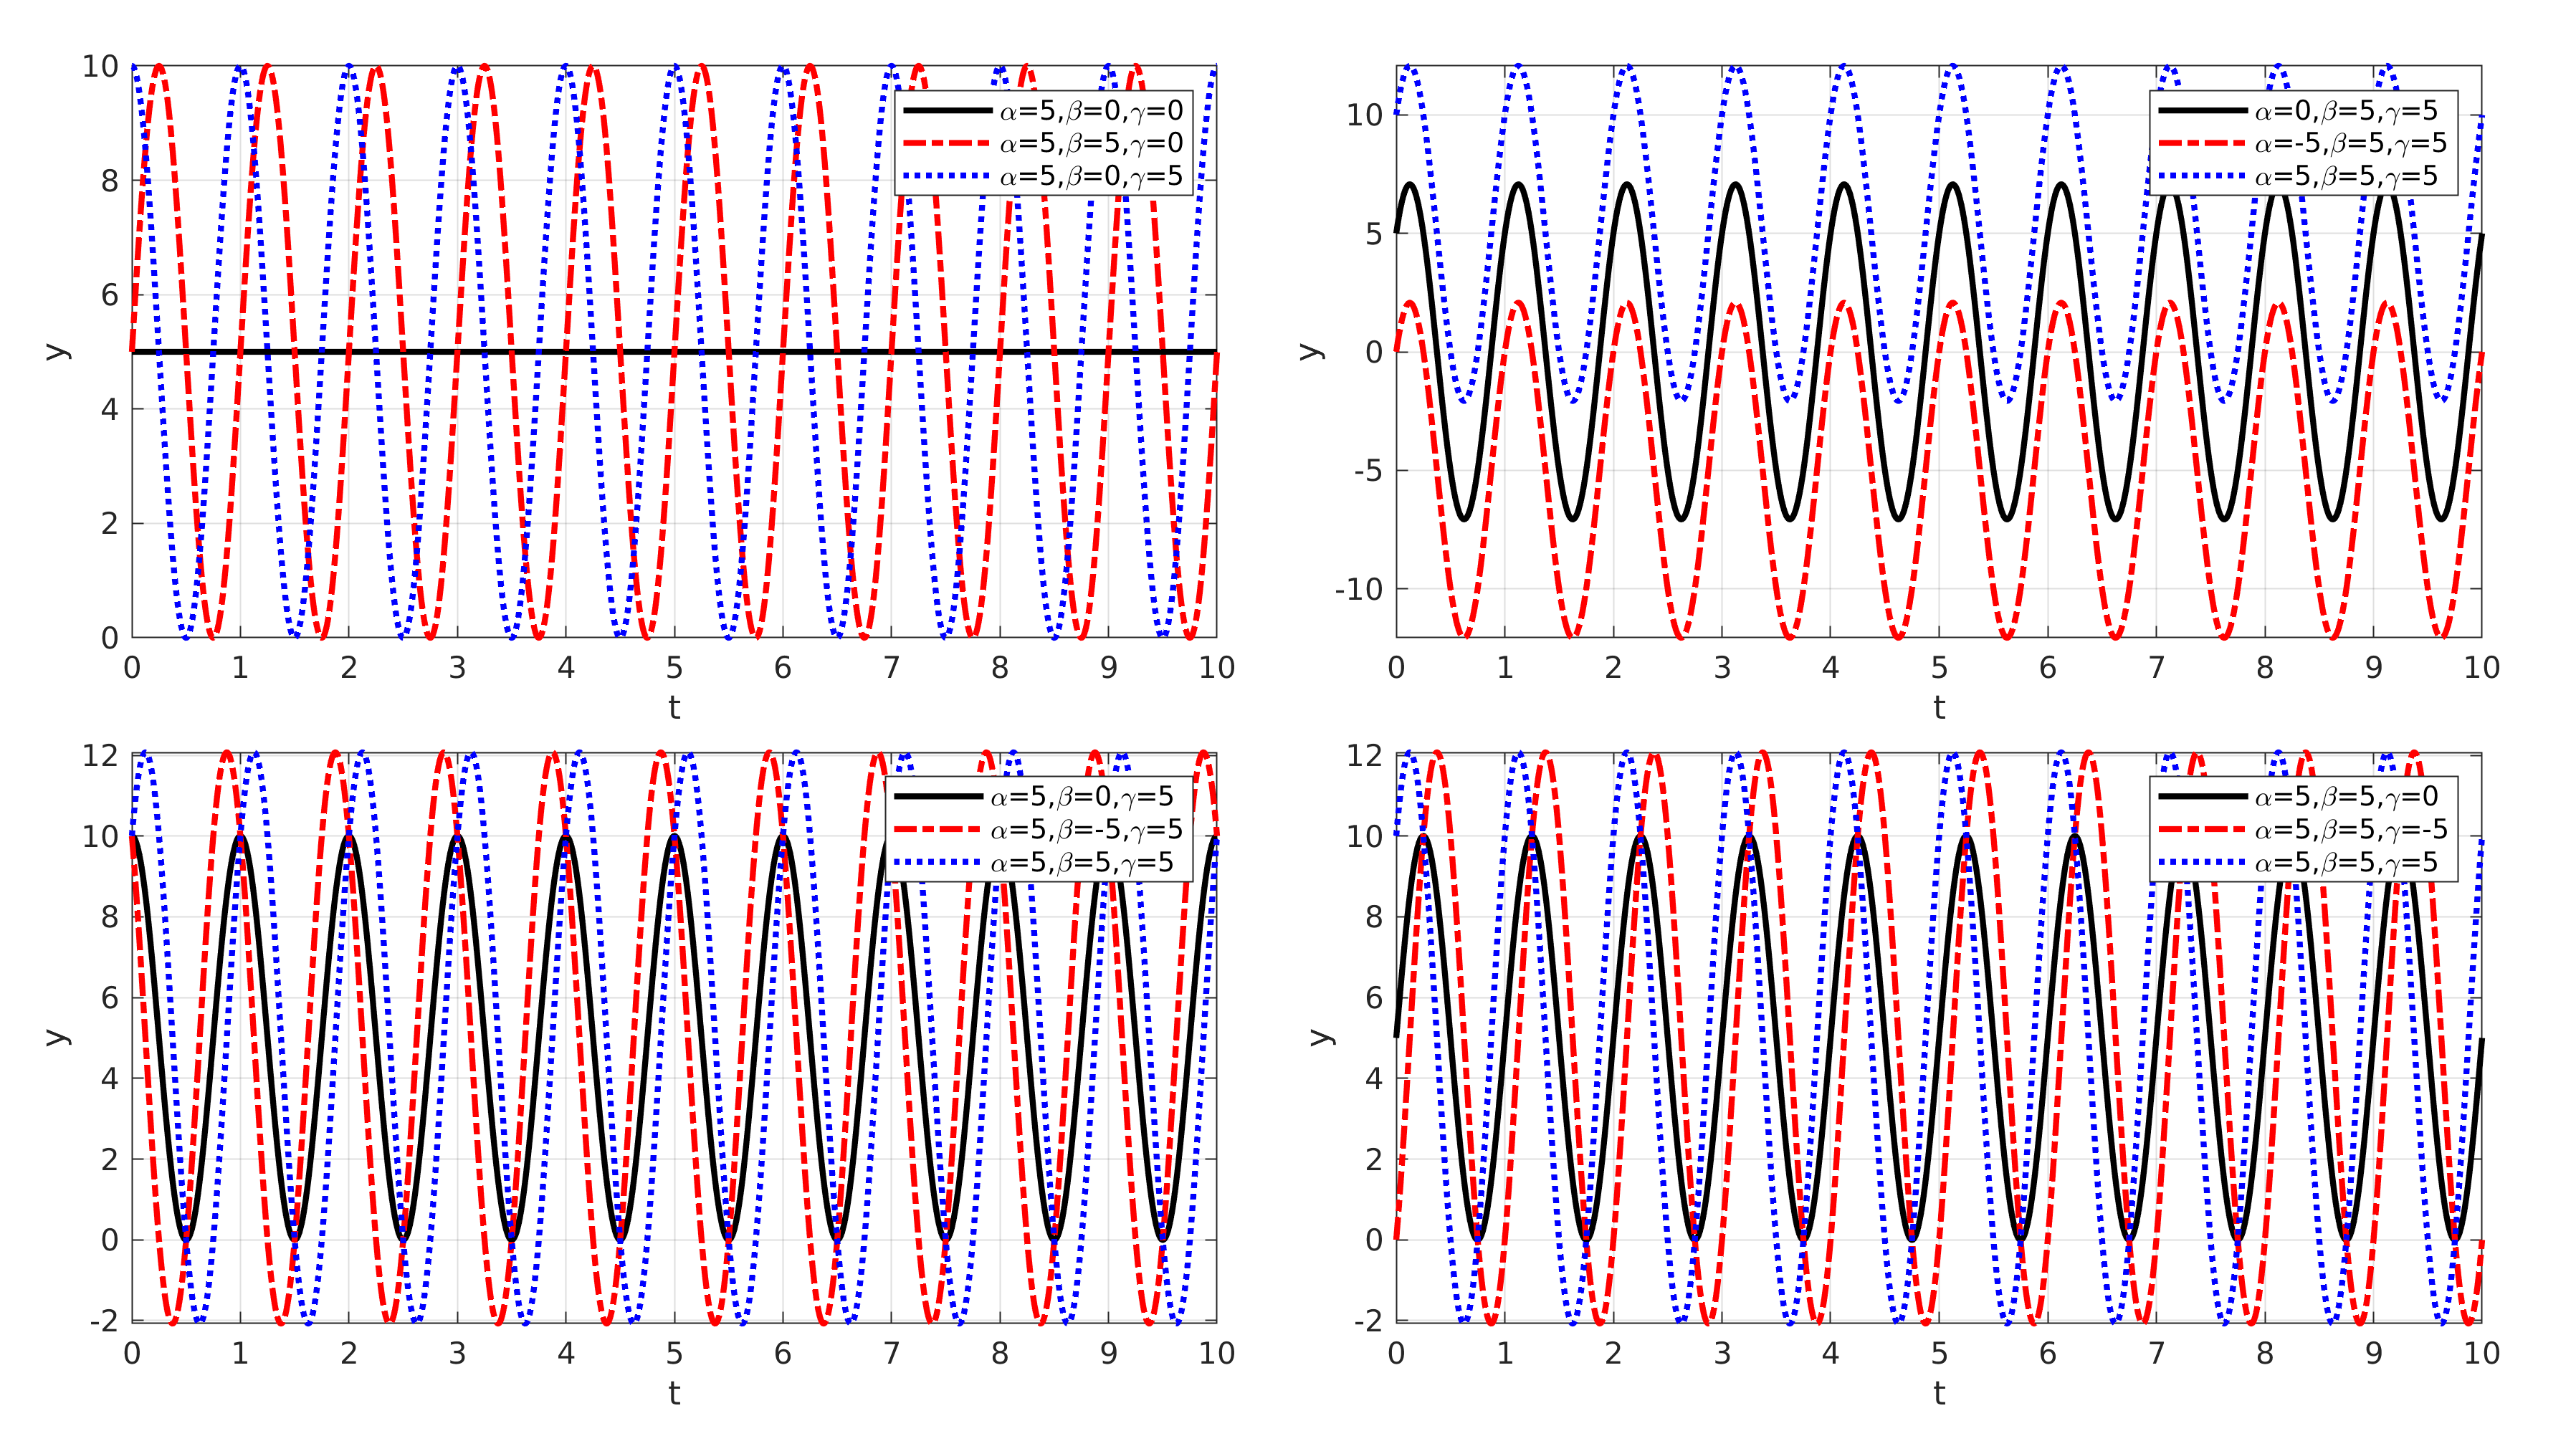
\includegraphics[width=15cm]{contents/Figures/sm_experiment}
		\caption{Kurva persamaan siklus musiman untuk beberapa nilai $\alpha,\beta$ dan $\gamma$.}
		\label{fig:sm}
	\end{figure}
	Gambar \ref{fig:sm} menampilkan ilustrasi persamaan \ref{eq:sm_} untuk nilai $\alpha,\beta$ dan $\gamma$ yang berbeda. Nilai $\alpha$ yang berbeda mempengaruhi posisi kurva terhadap sumbu-y. Sedangkan nilai $\beta$ dan $\gamma$ yang berbeda mempengaruhi posisi kurva terhadap sumbu-x.
\end{spacing}

